\subsection{Experimental Setup}

Our \gls{grasp} algorithm is implemented in C++20, leveraging modern language features for efficient memory management and performance. The implementation uses the Boost libraries for data structures and the Gurobi optimization suite for solving the MIP-based construction heuristics.

All computational experiments were conducted on a machine equipped with an Apple M1 Pro processor running macOS 24.5.0 (Darwin Kernel Version 24.5.0). The system architecture is ARM64, providing a modern computing environment for evaluating the algorithm's performance.

The complete implementation, along with all instances used in our experiments, is publicly available at \url{https://github.com/jsalvasoler/trigger_arc_tsp}.

\subsection{Metrics}

To evaluate the performance of our \gls{grasp} algorithm, we report the optimality gap, which measures how close our solutions are to the best possible solutions. The gap is calculated as:

\begin{equation}
\text{Gap} = \frac{\text{Solution Cost} - \text{Best Known Cost}}{\text{Best Known Cost}} \times 100\%
\end{equation}

For the competition instances (the first two datasets), we use the best known solutions provided by the competition organizers as the reference point.
For the synthetic instances (the third dataset), we use the best dual bound obtained after running the Gurobi MIP solver for one minute as the reference point, since optimal solutions are not known for these instances.
For construction heuristics, we also measure the success rate, i.e. the percentage of instances for which a solution was found.

\subsection{Gurobi Solver}


We use the Gurobi solver~\cite{gurobi} to solve the MIP model defined in~\ref{sec:mip_model}.
The competition instances are significantly harder than the synthetic instances, as shown in the Dataset report. In the context of MIP modeling, this is reflected in the fact
that Gurobi can only solve 6 / 21 instances of the C1 dataset, and 1 / 34 instances of the C2 dataset.
By solving, we mean that the solver was able to write the model in a reasonable time frame, and was able to provide a solution with a gap less than 1\% in under 5 hours.
For the other competition instances, the solver was not useful since it takes too long to write the model and does not provide feasible solutions or good bounds in reasonable times.
In many cases, the solver was running out of CPU memory.

Therefore, we only report the Gurobi results for the synthetic instances, in which we use a time limit of 1 minute and the default settings.

\begin{table}[h]
    \caption{Performance of Gurobi MIP solver on synthetic instances. Results show average computation time and optimality gap across different scenarios and problem sizes.}
    \label{tab:gurobi_performance}
    \centering
    \begin{tabular}{lrrrr}
        \toprule
        \textbf{Scenario} & \textbf{Nodes} & \textbf{Time (s)} & \textbf{Gap (\%)} \\
        \midrule
        \multirow{4}{*}{Balanced} & 10 & $1.89 \pm 2.81$ & $0.0 \pm 0.0$ \\
        & 15 & $24.04 \pm 28.83$ & $34.3 \pm 60.4$ \\
        & 20 & $34.95 \pm 29.40$ & $57.9 \pm 76.6$ \\
        & 25 & $40.84 \pm 24.70$ & $242.4 \pm 416.8$ \\
        \midrule
        \multirow{4}{*}{Decrease} & 10 & $3.90 \pm 7.38$ & $0.0 \pm 0.0$ \\
        & 15 & $25.13 \pm 27.40$ & $41.6 \pm 77.4$ \\
        & 20 & $40.14 \pm 26.30$ & $102.9 \pm 146.2$ \\
        & 25 & $48.38 \pm 19.54$ & $252.9 \pm 300.2$ \\
        \midrule
        \multirow{4}{*}{Increase} & 10 & $3.37 \pm 7.21$ & $0.0 \pm 0.0$ \\
        & 15 & $22.99 \pm 27.08$ & $36.8 \pm 83.6$ \\
        & 20 & $36.26 \pm 30.05$ & $97.1 \pm 161.7$ \\
        & 25 & $41.51 \pm 25.37$ & $154.8 \pm 215.0$ \\
        \bottomrule
    \end{tabular}
\end{table}

The three scenarios show similar behavior: all small instances (10 nodes) are solved to optimality, while both computation time and optimality gaps increase with problem size.
The Decrease scenario exhibits slightly higher gaps and longer runtimes compared to the other scenarios.

\subsection{Construction Heuristics Comparison}

\subsubsection{Randomized Greedy}
We run the Randomized Greedy construction heuristic (RGC) for a grid of values of the parameter $\alpha \in [0, 1]$. We run the RGC for 10 trials on each instance, and take the best solution found.
Recall that $\alpha \in [0, 1]$ controls the restricted candidate list (RCL) size, i.e. the fraction of the feasible edges that are considered in the greedy step, sorted by insertion cost.
Figure~\ref{fig:alpha_vs_mean_gap_randomized_greedy} shows the expected behavior of the RGC:
increasing values of $\alpha$ lead to higher gaps (since edge insertions are more expensive on average), but higher success rates (since more edges are considered).
The plot for dataset C2 shows some variability in the success rate, but we hypothesize that this behavior would dissapate with more trials.
The figure allows us to identify $\alpha = 0.1$ as a good choice for the RGC, as it provides a good balance between gap and success rate.
We will use this value for the rest of the experiments.

\begin{figure}[h]
    \centering
    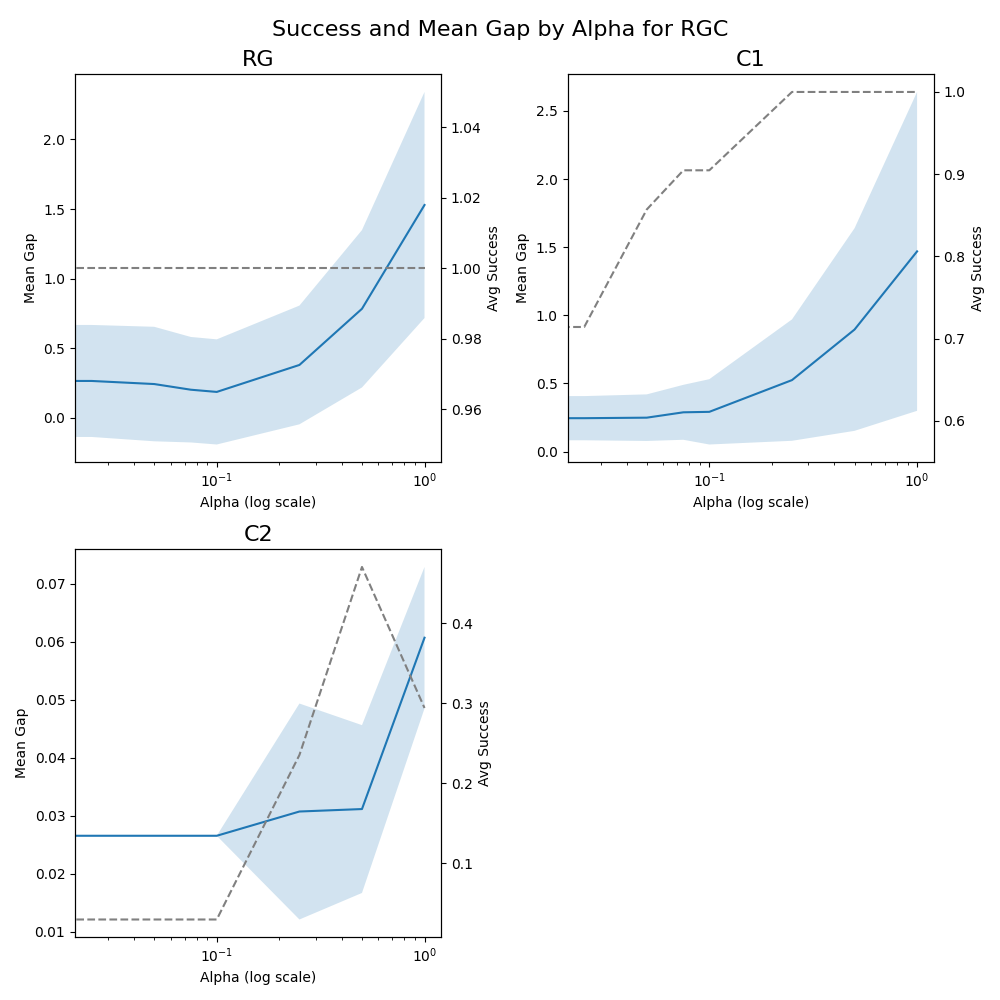
\includegraphics[width=0.49\textwidth]{figures/alpha_vs_mean_gap_randomized_greedy.png}
    \caption{Performance comparison of Randomized Greedy on synthetic instances. Results show average computation time (seconds) and optimality gap (\%) across different scenarios.}
    \label{fig:alpha_vs_mean_gap_randomized_greedy}
\end{figure}


\subsubsection{MIP Randomized Construction}

\paragraph{MIP-based Random Perturbation Construction}

We evaluate both additive ($\alpha$) and multiplicative ($\beta$) perturbation strategies for the MIP-based random perturbation construction heuristic across different parameter values.

\begin{table}[h]
    \caption{Performance of MIP Random Perturbation with additive noise ($\alpha$). Results show average optimality gap (\%) across different datasets and parameter values.}
    \label{tab:mip_alpha_results}
    \centering
    \setlength{\tabcolsep}{4pt}
    \begin{tabular}{lcccc}
        \toprule
        \textbf{Set} & \boldmath{$\alpha = 0.0$} & \boldmath{$\alpha = 0.1$} & \boldmath{$\alpha = 1.0$} & \boldmath{$\alpha = 10.0$} \\
        \midrule
        RG & $81.7 \pm 82.7$ & $70.9 \pm 75.6$ & $70.6 \pm 76.9$ & $\mathbf{68.9 \pm 75.3}$ \\
        C1 & $5.5 \pm 4.1$ & $\mathbf{4.3 \pm 3.2}$ & $7.3 \pm 3.9$ & $59.1 \pm 36.7$ \\
        C2 & $13.2 \pm 5.0$ & $\mathbf{6.6 \pm 2.2}$ & $7.0 \pm 2.4$ & $7.3 \pm 2.7$ \\
        \bottomrule
    \end{tabular}
\end{table}

\begin{table}[h]
    \caption{Performance of MIP Random Perturbation with multiplicative noise ($\beta$). Results show average optimality gap (\%) across different datasets and parameter values.}
    \label{tab:mip_beta_results}
    \centering
    \setlength{\tabcolsep}{4pt}
    \begin{tabular}{lcccc}
        \toprule
        \textbf{Set} & \boldmath{$\beta = 1.1$} & \boldmath{$\beta = 1.5$} & \boldmath{$\beta = 2.0$} & \boldmath{$\beta = 5.0$} \\
        \midrule
        RG & $\mathbf{69.1 \pm 72.8}$ & $70.7 \pm 76.0$ & $70.3 \pm 76.3$ & $69.9 \pm 74.6$ \\
        C1 & $4.9 \pm 4.2$ & $4.8 \pm 3.6$ & $\mathbf{4.3 \pm 3.2}$ & $4.4 \pm 3.9$ \\
        C2 & $6.6 \pm 2.7$ & $\mathbf{6.4 \pm 1.9}$ & $7.5 \pm 3.2$ & $6.9 \pm 2.8$ \\
        \bottomrule
    \end{tabular}
\end{table}

\subsubsection{MIP Biased Construction}

We evaluate the performance of the MIP-based biased construction heuristic
using the grid of values $\alpha \in [0.05, 0.1, 1.0, 3.0]$ and $\beta \in [0.05, 0.1, 1.0, 3.0]$.
Figure~\ref{fig:alpha_beta_grid_mip_randomized_construction_bias} shows the heatmap of average gaps across different $\alpha$ and $\beta$ combinations for each dataset.
The darker colors indicate better performance (lower gaps), allowing us to identify optimal parameter combinations for each dataset. 

For the RG and C1 datasets, higher values of $\alpha$ are better, while for the C2 dataset, lower values of $\beta$ are better. On all datasets, higher values of $\beta$ are better.
We will use the following parameter values for the rest of the experiments: $\alpha = 0.1$ and $\beta = 3.0$, which are a good trade-off in all datasets.

\begin{figure}[h]
    \centering
    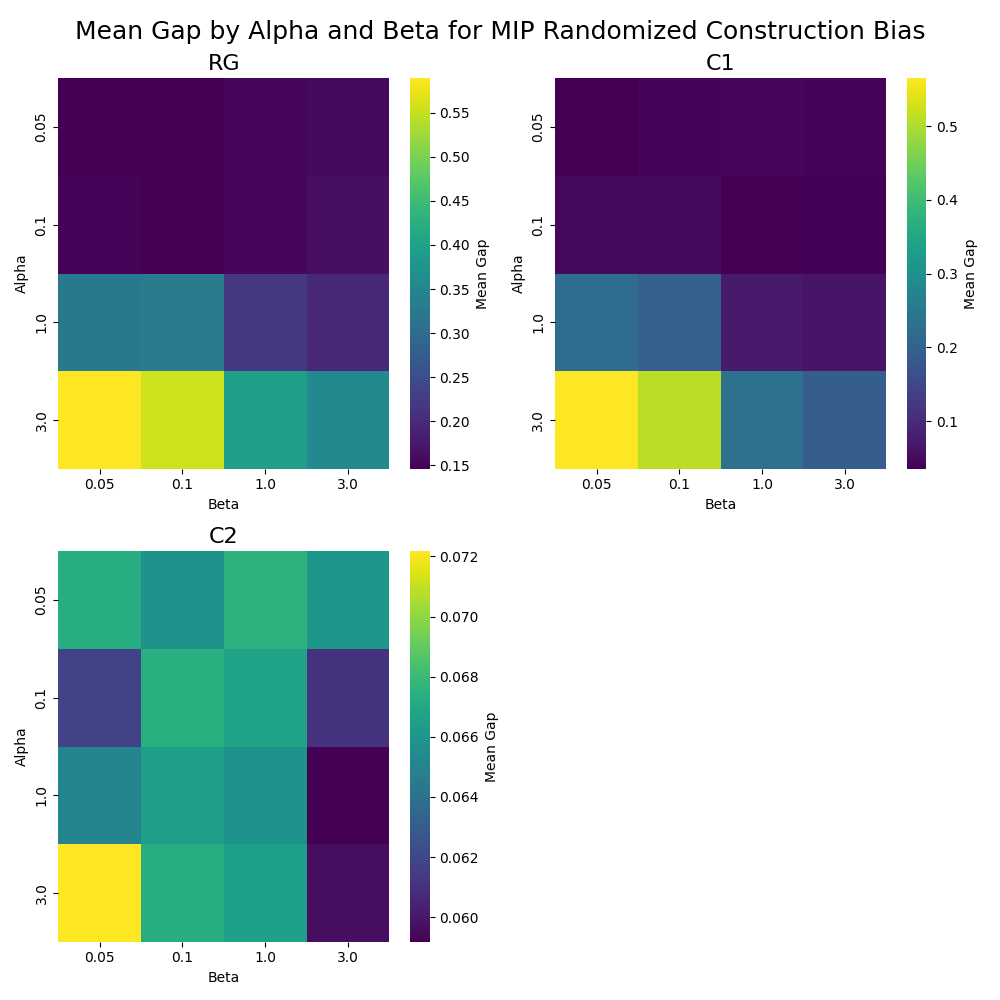
\includegraphics[width=0.49\textwidth]{figures/alpha_beta_grid_mip_randomized_construction_bias.png}
    \caption{Performance comparison of MIP Biased Construction with parameters $\alpha$ and $\beta$ on different datasets. Results show average optimality gap (\%) across different parameter combinations.}
    \label{fig:alpha_beta_grid_mip_randomized_construction_bias} 
\end{figure} 

\subsubsection{Comparison of Construction Heuristics}

We finally compare the performance of the tuned construction heuristics on all datasets.
We find that all datasets show the same ranking pattern: MIP Bias consistently achieves the best performance, followed by MIP $\alpha$-Rand and MIP $\beta$-Rand, with RGC and SRC performing significantly worse.
The MIP-based methods demonstrate superior solution quality across all datasets, with gaps ranging from 3.8\% to 6.6\% on competition instances (C1, C2) and around 70\% on synthetic instances (RG).
In contrast, the simpler heuristics (SRC, RGC) show much higher gaps, particularly on the RG dataset where SRC reaches nearly 300\% gap. Notably, SRC fails completely on C2 (0\% success rate), while RGC shows poor performance on C2 (2.9\% success rate).
The MIP methods maintain 100\% success rates because finding feasibility for the TSP is easy on our datasets. Runtime analysis reveals that SRC and RGC are the fastest (under 0.1 seconds), while MIP methods require 1-6 seconds, with MIP approaches taking a bit longer.
However, all methods except for Gurobi are fast enough to be used in a real-time application, which is one of our main goals.
Given these results, the construction heuristic that we will use in the GRASP framework is MIP Bias.


\begin{table}[h]
    \caption{Performance comparison of construction heuristics across all datasets. Results show average gap (\%), runtime (seconds), and success rate for each method-dataset combination.}
    \label{tab:construction_comparison}
    \centering
    \setlength{\tabcolsep}{2.1pt}
    \begin{tabular}{llrrr}
        \toprule
        \textbf{Set} & \textbf{Method} & \textbf{Gap (\%)} & \textbf{Time (s)} & \textbf{Success} \\
        \midrule
        \multirow[c]{6}{*}{C1} & SRC & $163.6 \pm 128.5$ & $0.0 \pm 0.0$ & $0.95$ \\
        & RGC ($\alpha = 0.1$) & $29.2 \pm 24.6$ & $0.1 \pm 0.1$ & $0.91$ \\
        & MIP $\alpha$-Rand(0.1) & $4.3 \pm 3.2$ & $3.2 \pm 3.7$ & $1.00$ \\
        & MIP $\beta$-Rand(1.5) & $4.8 \pm 3.7$ & $3.2 \pm 3.4$ & $1.00$ \\
        & MIP Bias(0.1, 3.0) & $\mathbf{3.8 \pm 2.8}$ & $4.1 \pm 5.2$ & $1.00$ \\
        \midrule
        \multirow[c]{6}{*}{C2} & SRC & $-$ & $0.0 \pm 0.0$ & $0.00$ \\
        & RGC ($\alpha = 0.1$) & $2.7$ & $1.5 \pm 1.7$ & $0.03$ \\
        & MIP $\alpha$-Rand(0.1) & $6.6 \pm 2.2$ & $6.1 \pm 3.8$ & $1.00$ \\
        & MIP $\beta$-Rand(1.5) & $6.4 \pm 1.9$ & $5.9 \pm 3.7$ & $1.00$ \\
        & MIP Bias(0.1, 3.0) & $\mathbf{6.1 \pm 1.8}$ & $1.9 \pm 1.5$ & $1.00$ \\
        \midrule
        \multirow[c]{6}{*}{RG} & Gurobi & $85.1 \pm 192.5$ & $26.9 \pm 27.5$ & $1.00$ \\
        & SRC & $296.4 \pm 236.0$ & $0.0 \pm 0.0$ & $1.00$ \\
        & RGC ($\alpha = 0.1$) & $66.8 \pm 59.0$ & $0.0 \pm 0.0$ & $1.00$ \\
        & MIP $\alpha$-Rand(0.1) & $70.9 \pm 75.8$ & $1.1 \pm 1.9$ & $1.00$ \\
        & MIP $\beta$-Rand(1.5) & $70.7 \pm 76.2$ & $1.1 \pm 1.9$ & $1.00$ \\
        & MIP Bias(0.1, 3.0) & $\mathbf{69.7 \pm 75.1}$ & $1.1 \pm 1.8$ & $1.00$ \\
        \bottomrule
    \end{tabular}
\end{table}
